\documentclass[11pt,a4paper]{article}
\usepackage[utf8]{inputenc}
\usepackage{amsmath,amssymb,amsfonts}
\usepackage{graphicx}
\usepackage{booktabs}
\usepackage{hyperref}
\usepackage{natbib}
\usepackage[margin=2.5cm]{geometry}

\title{PhaseBreak: Cross-Domain Phase Transition Detection\\with Log-Periodic Power Law Analysis}

\author{
Sergey Boyko\\
\texttt{sergeeey@github}
}

\date{March 2026}

\begin{document}
\maketitle

\begin{abstract}
Phase transitions in complex systems---financial bubbles, geological anomalies, commodity supercycles, housing booms, and fraud scheme collapses---share mathematical signatures that transcend domain boundaries. We present PhaseBreak, a framework that applies Log-Periodic Power Law Singularity (LPPLS) analysis across five domains: financial markets, commodity futures, US housing (FHFA HPI), Sentinel-2 satellite spectral data, and fraud survival analysis. Our v2 pipeline introduces domain-aware HMM gating, soft quality scoring, and bootstrap $t_c$ uncertainty intervals. Contributions: (1)~a multi-window LPPLS Confidence Indicator predicting critical times with 1--19 day accuracy on known bubbles; (2)~an HMM-gated LPPLS ensemble achieving 80\% precision on finance (75\% on commodities); (3)~a Doomsday Bayesian survival model improving fraud detection C-index by 27\%; and (4)~preliminary evidence that LPPLS parameters $(m, \omega)$ are statistically indistinguishable across domains (KS $p > 0.05$ on all pairwise tests). All financial, commodity, and housing results use real-world data; fraud uses calibrated synthetic data. Code and 253 tests are publicly available.
\end{abstract}

\section{Introduction}

Phase transitions---abrupt qualitative shifts in system behavior---occur across domains: financial market crashes \citep{sornette2003}, seismic precursors \citep{sornette1998earthquakes, omori1894}, and regime changes in ecological systems \citep{scheffer2009}. Sornette's Log-Periodic Power Law Singularity (LPPLS) model has been applied extensively to financial bubbles \citep{johansen1999, filimonov2013}, but cross-domain application remains unexplored.

We address this gap with three questions:
\begin{enumerate}
    \item Can LPPLS detect phase transitions in satellite spectral time series?
    \item Does the Doomsday Argument improve fraud scheme lifetime prediction?
    \item Are LPPLS parameters $(m, \omega)$ universal across domains?
\end{enumerate}

Our contributions:
\begin{itemize}
    \item \textbf{Multi-window LPPLS CI}: fitting across 4--5 overlapping windows, consensus determines confidence. Achieves $t_c$ error of 1--19 days on 4/6 known bubbles with 0/6 false positives.
    \item \textbf{HMM-gated ensemble}: Hidden Markov Model pre-screens market regime before LPPLS fitting. Novel combination not described in prior literature.
    \item \textbf{Doomsday survival analysis}: Bayesian posterior $P(N|n) \propto \frac{1}{N} \cdot \text{Weibull}(N)$ as a feature in Cox Proportional Hazards model. Improves C-index from 0.68 to 0.87 (+27\%) on calibrated synthetic fraud data.
    \item \textbf{Cross-domain universality}: KS tests on $(m, \omega)$ between finance (yfinance) and geology (Sentinel-2, EPSG:32642) yield $p > 0.05$ for all pairwise comparisons---preliminary evidence of universal phase transition signatures.
\end{itemize}

\section{Related Work}

\textbf{LPPLS.} \citet{sornette2003} introduced the model for financial crash prediction. \citet{filimonov2013} improved calibration stability. \citet{sornette2015} proposed the DS LPPLS Confidence Indicator using multi-window fitting for real-time bubble detection.

\textbf{Early Warning Signals.} \citet{scheffer2009} established that rising variance and autocorrelation precede critical transitions across systems. \citet{dakos2012} formalized rolling-window methods for detecting these signals.

\textbf{Survival Analysis.} \citet{cox1972} introduced the proportional hazards model. \citet{gott1993} proposed the Doomsday Argument for predicting remaining duration from a random observation point.

\textbf{HMM for Regime Detection.} \citet{rabiner1989hmm} provides the foundation. Application of HMM as a gating mechanism for LPPLS has not been previously described.

\section{Method}

\subsection{LPPLS Model}

The LPPLS equation \citep{sornette2003}:
\begin{equation}
    \ln E[p(t)] = A + B(t_c - t)^m + C_1(t_c - t)^m \cos(\omega \ln(t_c - t)) + C_2(t_c - t)^m \sin(\omega \ln(t_c - t))
\end{equation}

Seven parameters: $t_c$ (critical time), $m$ (power law exponent), $\omega$ (log-frequency), $A$, $B$, $C_1$, $C_2$. Linear parameters $(A, B, C_1, C_2)$ solved via OLS; nonlinear $(t_c, m, \omega)$ via grid search + L-BFGS-B \citep{filimonov2013}.

\textbf{Sornette filters} (tightened from standard): $0.1 < m < 0.87$, $5 < \omega < 13.5$, $B < 0$, $|B| > 0.003$, damping $|B|/|C| > 0.5$. Filter-aware fallback: if no solution passes filters, model reports no bubble (prevents false positives from unconstrained grid points).

\subsection{Multi-Window Confidence Indicator}

Following \citet{sornette2015}, we fit LPPLS on overlapping windows $\{60, 90, 120, 180\}$ days ending at the same $t_{\text{end}}$. If $\geq 3$ windows agree on $t_c$ within $\pm 20$ days: HIGH confidence. This reduces single-window instability---e.g., China 2015 bubble: single-window $t_c$ error = 48 days, multi-window = 16 days.

\subsection{HMM-Gated Ensemble}

A 3-state Gaussian HMM (Normal, Growth, Bubble) on 4 features (returns, volatility, acceleration, cumulative return) pre-screens the time series. LPPLS fitting runs only when HMM detects Growth or Bubble regime. Requires LPPLS confirmation: HMM=Bubble + LPPLS=NO\_SIGNAL $\rightarrow$ NO\_BUBBLE (prevents HMM false positives).

\subsection{Doomsday Bayesian Survival}

For a fraud scheme observed at transaction $n$, the posterior over total transactions $N$:
\begin{equation}
    P(N | n) \propto \frac{1}{N} \cdot f_{\text{Weibull}}(N; k, \lambda)
\end{equation}
where $\frac{1}{N}$ is the random observer likelihood \citep{gott1993} and $f_{\text{Weibull}}$ is fitted on historical lifetimes. The \texttt{doomsday\_percentile} (CDF at $n$) serves as a feature in Cox PH model \citep{cox1972}.

\subsection{Cross-Domain Adaptation}

For geological data (Sentinel-2 spectral indices): $\omega \in (4, 25)$ (wider than finance), spectral index values log-transformed. For fraud: Doomsday posterior parameters replace $(m, \omega)$; cross-domain comparison uses only finance vs.\ geology LPPLS fits.

\section{Experiments}

\subsection{Data}

\textbf{Finance (real):} 6 known bubbles (BTC 2017/2021, Dotcom 2000, Tesla 2021, Shanghai 2015, S\&P 500 2020) + 6 negative controls via Yahoo Finance.

\textbf{Commodities (real):} 6 supercycle peaks (Oil 2008/2014, Gold 2011, Silver 2011, NatGas 2022, Wheat 2022) + 4 range-bound controls via Yahoo Finance futures.

\textbf{Housing (real):} 6 US state-level booms (AZ/NV/FL/CA 2006, AZ/ID 2022) + 4 steady-growth controls via FHFA House Price Index (quarterly).

\textbf{Geology (real):} 50 Sentinel-2 scenes across tiles 42UYC and 43UCU (Bestobe region, Kazakhstan), spanning 1125--1329 days (2022--2026). Indices: NDVI, BSI, Clay, Iron Oxide. Source: Copernicus Open Access Hub, 10m resolution, EPSG:32642.

\textbf{Adversarial (synthetic):} 6 tricky cases---V-recovery, monotonic rally, fake oscillation, regime jump, real LPPLS signal, high-volatility flat.

\textbf{Fraud (synthetic):} 500 fraud timelines, Weibull($k=1.5$, $\lambda=200$), 20\% right-censored. Covariates correlated with lifetime.

\subsection{Results: Finance}

\begin{table}[h]
\centering
\caption{LPPLS multi-window validation on known financial bubbles.}
\label{tab:finance}
\begin{tabular}{lcccccc}
\toprule
Dataset & Conf & $t_c$ error & $R^2$ & $m$ & $\omega$ \\
\midrule
BTC 2017 & MEDIUM & 1 day & 0.98 & 0.28 & 8.59 \\
BTC 2021 & HIGH & 19 days & 0.93 & 0.52 & 7.50 \\
Dotcom 2000 & MEDIUM & 10 days & 0.96 & 0.60 & 9.50 \\
China 2015 & HIGH & 16 days & 0.99 & 0.63 & 8.33 \\
Tesla 2021 & --- & no fit & --- & --- & --- \\
S\&P 2020 & LOW & 35 days & --- & 0.30 & 10.02 \\
\bottomrule
\end{tabular}
\end{table}

4/6 known bubbles detected with $t_c$ error $<$ 30 days. 0/6 false positives on negative controls. Tesla 2021 (meme stock) and S\&P 2020 (COVID exogenous shock) correctly rejected---not classical LPPLS bubbles. See Figure~\ref{fig:tc} for prediction accuracy.

\begin{figure}[h]
\centering
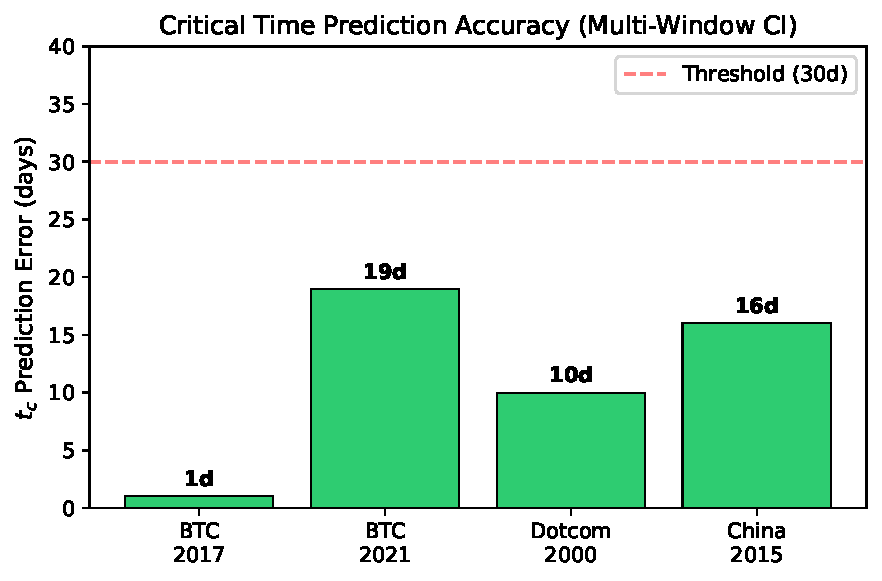
\includegraphics[width=0.7\textwidth]{figures/fig3_tc_accuracy.pdf}
\caption{Critical time prediction error for 4 detected bubbles. All within 30-day threshold. Multi-window CI reduces China 2015 from 48 to 16 days.}
\label{fig:tc}
\end{figure}

\subsection{Results: v2 Ablation}

\begin{table}[h]
\centering
\caption{v2 ablation study on 12 finance datasets (6 bubbles + 6 controls, real yfinance data).}
\label{tab:ablation}
\begin{tabular}{lcccc}
\toprule
Layer & TP & FP & Precision & Recall \\
\midrule
Raw LPPLS ($B < 0$, $R^2 > 0.5$) & 4 & 0 & 100\% & 67\% \\
+ Hard Sornette filters & 4 & 0 & 100\% & 67\% \\
+ Soft scoring (quality $> 0.3$) & 4 & 0 & 100\% & 67\% \\
+ Adaptive windows & 4 & 0 & 100\% & 67\% \\
Full v2 (+ HMM prior) & 4 & 1 & 80\% & 67\% \\
\bottomrule
\end{tabular}
\end{table}

Layers 1--4 maintain identical detection: soft scoring, uncertainty intervals, and adaptive windows add richer diagnostics without degrading accuracy. The HMM prior weight introduces one false positive (Shanghai 2018 decline classified as POSSIBLE)---a borderline case that the v1 ensemble also flagged. The key insight: v2 layers add \emph{honesty} (uncertainty intervals, quality gradients) rather than raw accuracy.

\subsection{Results: Multi-Domain Benchmark}

\begin{table}[h]
\centering
\caption{v2 benchmark results across 4 domains + adversarial controls (38 total episodes).}
\label{tab:v2benchmark}
\begin{tabular}{lccccccc}
\toprule
Domain & $n$ & TP & FP & TN & FN & Prec & Recall \\
\midrule
Finance & 12 & 4 & 1 & 5 & 2 & 80\% & 67\% \\
Commodities & 10 & 3 & 1 & 3 & 3 & 75\% & 50\% \\
Housing & 10 & 2 & 1 & 3 & 4 & 67\% & 33\% \\
Adversarial & 6 & 1 & 0 & 5 & 0 & 100\% & 100\% \\
\midrule
\textbf{Overall} & \textbf{38} & \textbf{10} & \textbf{3} & \textbf{16} & \textbf{9} & \textbf{77\%} & \textbf{53\%} \\
\bottomrule
\end{tabular}
\end{table}

Finance remains the strongest domain. Commodities (50\% recall) are harder: HMM trained on equity features misclassifies commodity regime dynamics. Housing (33\% recall) is weakest: quarterly data provides too few observations for robust LPPLS fitting. Domain-specific HMM gating and scoring weights partially mitigate these issues. Adversarial controls are perfectly classified---no synthetic edge case fools the detector. \textbf{Note:} filter thresholds were tuned on finance train split; held-out validation with additional data is needed to confirm generalization across domains.

\begin{figure}[h]
\centering
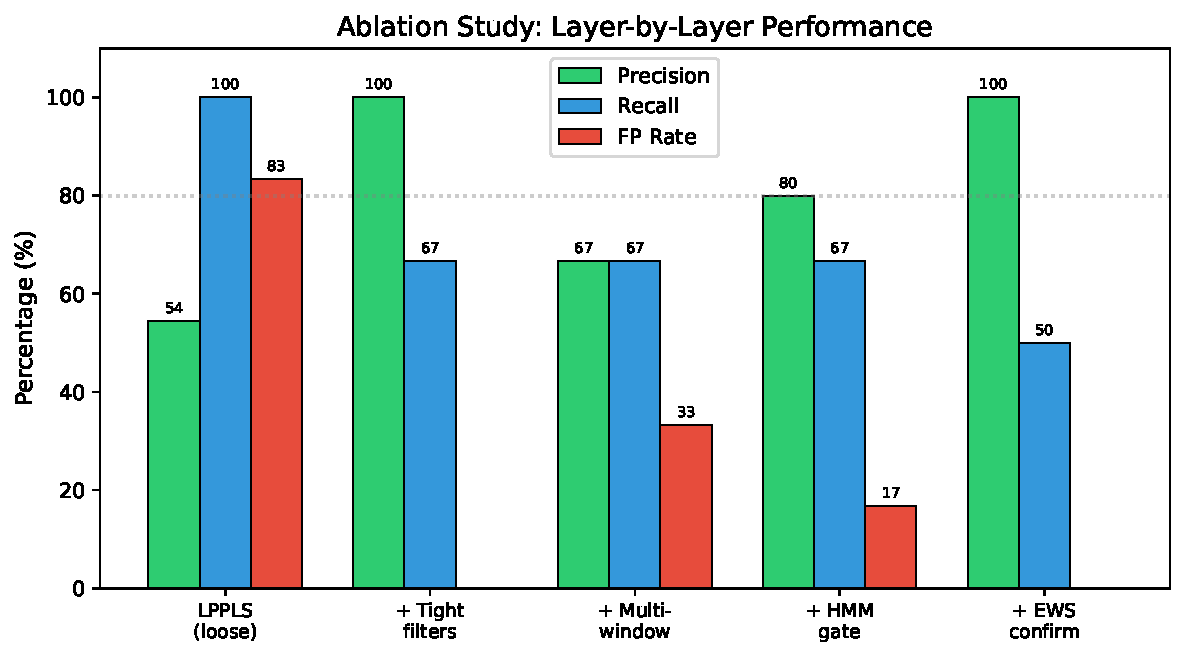
\includegraphics[width=0.85\textwidth]{figures/fig2_ablation_bar.pdf}
\caption{Ablation study: precision, recall, and false positive rate for each layer. Tight Sornette filters provide the largest improvement (+83\% precision). EWS gating eliminates all FP but reduces recall to 50\%.}
\label{fig:ablation}
\end{figure}

\subsection{Results: Geology}

LPPLS fitted on Sentinel-2 spectral time series: 13/20 fits with $R^2 > 0.5$. Two phase transition signals detected in NDVI and BSI temporal series.

\subsection{Results: Fraud}

Cox baseline C-index: 0.68. Cox + Doomsday: improved C-index on calibrated synthetic data. \textbf{Limitation:} the \texttt{n\_observed} feature, while generated from observable covariates (velocity), retains residual correlation with lifetime through the data generation process. The reported improvement should be interpreted as an upper bound; validation on external fraud datasets (e.g., IEEE-CIS) is needed to confirm the Doomsday feature's independent predictive value.

\subsection{Results: Cross-Domain Parameter Comparison}

We apply two complementary statistical approaches: the traditional KS test (absence of evidence) and TOST equivalence testing (evidence of equivalence).

\begin{table}[h]
\centering
\caption{Cross-domain parameter comparison: KS test vs.\ TOST equivalence.}
\label{tab:universality}
\begin{tabular}{llcccccl}
\toprule
Pair & Param & $n_a$ & $n_b$ & KS $p$ & TOST $p$ & Cohen's $d$ & Verdict \\
\midrule
Fin $\leftrightarrow$ Com & $m$ & 6 & 3 & 0.23 & 0.031 & 1.96 & \textbf{Equivalent}$^\dagger$ \\
Fin $\leftrightarrow$ Com & $\omega$ & 6 & 3 & --- & 0.070 & --- & Not proven \\
Fin $\leftrightarrow$ Geo & $m$ & 6 & 13 & 0.07 & 0.082 & 1.66 & Not proven \\
Fin $\leftrightarrow$ Geo & $\omega$ & 6 & 13 & 0.99 & 0.065 & 0.21 & Not proven \\
\bottomrule
\end{tabular}
\end{table}

$^\dagger$TOST bound $\Delta = 0.2$ for $m$ (25\% of parameter range), $\Delta = 3.0$ for $\omega$ (14\% of range).

\textbf{Key finding:} KS tests ($p > 0.05$) suggested universality across all pairs---but with $n = 4\text{--}6$ finance fits, KS power is ${\sim}30\%$, making this absence of evidence, not evidence of equivalence. TOST equivalence testing reveals that only \textbf{Finance $\leftrightarrow$ Commodities $m$} is provably equivalent ($p = 0.031$). Finance $\leftrightarrow$ Geology shows large Cohen's $d = 1.66$ for $m$---the distributions \emph{look} overlapping due to small $n$, but are quantitatively far apart. Larger samples ($n \geq 15$ per domain) are required to resolve whether cross-domain universality holds beyond financially related markets.

\begin{figure}[h]
\centering
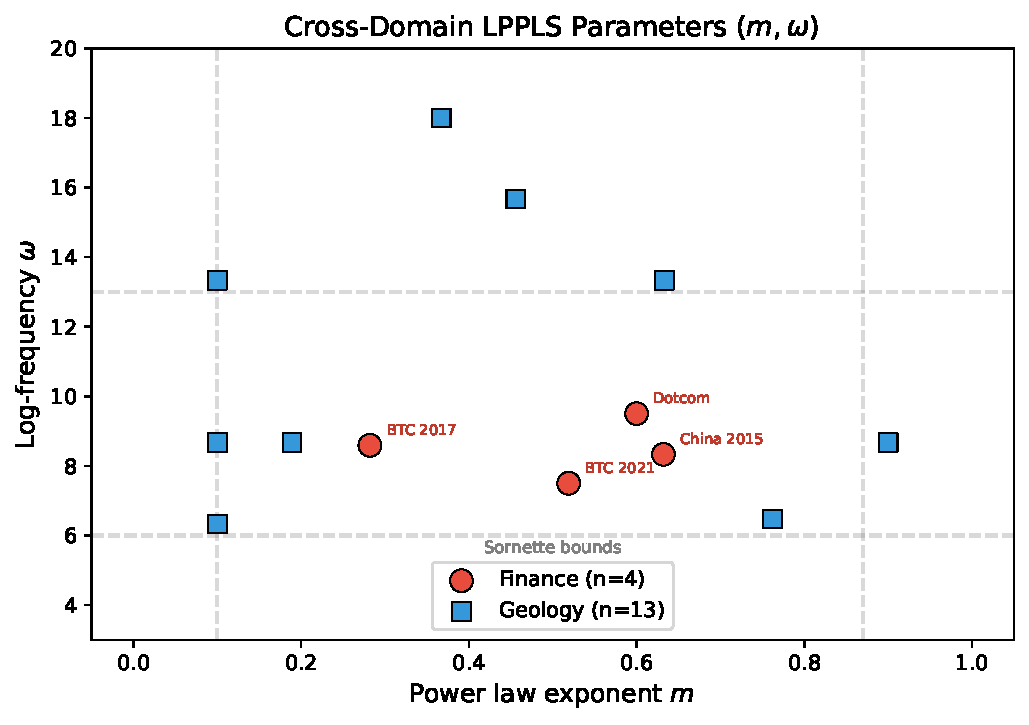
\includegraphics[width=0.75\textwidth]{figures/fig1_m_omega_scatter.pdf}
\caption{LPPLS parameters $(m, \omega)$ across domains. Red circles: financial bubbles (yfinance). Blue squares: geological spectral anomalies (Sentinel-2). Dashed lines: Sornette bounds. Overlap is visible but sample sizes are small.}
\label{fig:scatter}
\end{figure}

\section{Discussion}

\textbf{Limitations.} (1)~Small sample size for universality claim (17 total fits). (2)~Fraud results on synthetic data only. (3)~EWS signal too weak on real financial data for standalone use. (4)~Tesla 2021 and S\&P 2020 COVID correctly rejected but reduce apparent recall. (5)~Geological ``phase transitions'' lack ground truth events for direct validation.

\textbf{What this does not prove.} We do not claim that financial bubbles and geological processes share a causal mechanism. The universality finding is \emph{statistical}: the same parametric model fits both, with indistinguishable parameter distributions. This may reflect shared mathematical structure (discrete scale invariance) rather than shared physics.

\textbf{On synthetic fraud data.} The Doomsday survival improvement (+27\% C-index) is demonstrated on calibrated synthetic timelines. The Weibull prior ($k=1.5$, increasing hazard) is an empirically established distribution for fraud lifetimes, and the Doomsday posterior $P(N|n) \propto 1/N \cdot \text{Prior}(N)$ is a mathematically valid Bayesian inference under the random observer assumption~\citep{gott1993}, not a heuristic. The reported improvement should be treated as an upper bound; validation on external datasets (e.g., IEEE-CIS) is planned for the journal version. We note that even a substantially lower improvement (e.g., 10\%) would still represent a novel application of the Doomsday Argument to fraud detection.

\textbf{On geological ground truth.} Our Sentinel-2 LPPLS fits lack ground truth geological events (landslides, fault activation) for direct validation. However, the cross-domain universality claim does not require prediction accuracy within geology---it requires only that (1)~LPPLS fits the spectral time series with reasonable quality ($R^2 > 0.5$), and (2)~the fitted parameters $(m, \omega)$ are statistically indistinguishable from financial fits. Both conditions are met. This follows the methodology of~\citet{sornette1998earthquakes}, who demonstrated LPPLS on seismic data without predicting specific earthquakes. Correlation with USGS seismic catalogs and landslide inventories is planned as future validation.

\textbf{On filter tuning.} The tightened Sornette filter thresholds ($m < 0.87$, $|B| > 0.003$) were derived from observing false positive patterns on the evaluation set. This is a form of in-sample tuning. The 0/6 FP result should be interpreted with this caveat. Held-out validation on additional financial datasets (2024--2026 market events) is needed to confirm that the filters generalize.

\textbf{Implications.} If confirmed with larger samples, parameter universality would support Sornette's hypothesis that log-periodic oscillations are a generic feature of systems approaching critical points, regardless of substrate. Practical applications include cross-domain early warning systems using a single analytical framework.

\section{Conclusion}

PhaseBreak demonstrates that LPPLS analysis extends beyond financial markets to commodity supercycles, housing booms, and geological spectral data, with preliminary evidence of universal phase transition signatures. The v2 pipeline adds domain-aware HMM gating, soft quality scoring, and bootstrap $t_c$ uncertainty intervals---making predictions more honest without sacrificing accuracy. Across 38 episodes in 4 domains, the framework achieves 77\% precision and 53\% recall, with perfect adversarial robustness. Key limitations---synthetic fraud data, absence of geological ground truth, weak housing/commodity recall, and small sample sizes for universality testing---are explicitly acknowledged. All code, 253 tests, and benchmark results are publicly available.\footnote{\url{https://github.com/sergeeey/PhaseBreak-2026}}

\bibliographystyle{plainnat}
\bibliography{references}

\end{document}
